\chapter{Usage}
\label{sec:usage}

\section{Introduction}
% TODO

\section{Installation}
% TODO

Note: At present, no binary or source distributions are available yet.
The following sections were written in anticipation of the future release of the BlasterSim beta version.

\subsection{System requirements}

BlasterSim is written in Fortran 2018 and will run on any computer a modern Fortran compiler allows.
BlasterSim has no dependencies.

\subsection{Installation from binaries}
\label{sec:installation from binaries}

Obtain the latest BlasterSim binary from \url{http://trettel.us/blastersim/releases/}.
For Linux, this is blastersim-\gittag-linux.tgz.
For Windows, this is blastersim-\gittag-windows.zip.
For macOS, this is blastersim-\gittag-mac.tgz.

The \texttt{blastersim} executable on Linux and macOS and the \texttt{blastersim.exe} executable on Windows can either be placed in the directory you want to run BlasterSim from or placed on your \texttt{PATH}.

\subsection{Installation from source tarball}
\label{sec:installation from source tarball}

Obtain the latest BlasterSim source code from \url{http://trettel.us/blastersim/releases/blastersim-\gittag-source.zip}.

The provided source code has no dependencies other than a modern Fortran compiler and a Make program like GNU Make on Linux and macOS or \href{https://wiki.qt.io/Jom}{jom} or \href{https://learn.microsoft.com/en-us/cpp/build/reference/nmake-reference?view=msvc-170}{NMAKE} on Windows.
Unfortunately, BlasterSim will not compile with every Fortran compiler due to the units module being too large.
BlasterSim will compile with gfortran and for that reason gfortran is recommended.

After extracting the provided source archive, \texttt{cd} into the directory and build BlasterSim.

On Linux and macOS you can type \texttt{make BUILD=release blastersim}.

On Windows you can type (if using jom) \texttt{jom BUILD=release blastersim.exe}

Note that compilation of BlasterSim can be slow.

Once built, a BlasterSim executable should be moved to a directory on your \texttt{PATH} as discussed in \secref{installation from binaries}.

\subsection{Installation from clone of Git repository}
% TODO

Building from the Git repository requires first building genunits from Ben Trettel's \href{https://github.com/btrettel/flt/}{FLT} repository.
The requirement for a modern Fortran compiler remains the same as that from \secref{installation from source tarball}.

On Linux and macOS, clone the FLT repository and build genunits:
\begin{verbatim}
git clone https://github.com/btrettel/flt.git
cd flt
make BUILD=release genunits geninput
\end{verbatim}

On Windows with jom, you should replace \texttt{make genunits geninput} with \texttt{jom genunits.exe geninput.exe}.

Place \texttt{genunits} or \texttt{genunits.exe} on your \texttt{PATH}.
Now you can build BlasterSim by cloning the BlasterSim repository, \texttt{cd}ing into the clone, and following the instructions in \secref{installation from source tarball}.
To be more specific for GNU Make for Linux and macOS:
\begin{verbatim}
git clone https://github.com/btrettel/blastersim.git
cd blastersim
make BUILD=release blastersim
\end{verbatim}

On Windows with jom, you should replace \texttt{make BUILD=release blastersim} with \texttt{jom BUILD=release blastersim.exe}.

And again, a BlasterSim executable should be moved to a directory on your \texttt{PATH} as discussed in \secref{installation from binaries}.

\section{BlasterSim inputs in general}
% TODO

BlasterSim uses Fortran namelist format input files.

% <https://www.intel.com/content/www/us/en/docs/fortran-compiler/developer-guide-reference/2023-0/namelist.html>
% TODO: Discuss namelist input files in general

% TODO: Example namelist

BlasterSim uses SI units in its input files and internally.
Support for other unit systems is not planned at the moment due to the complexity of supporting multiple unit systems.
Scientific notation can be used to appropriately scale inputs. For example, instead of 13 mm being written as \texttt{0.013} m, the user can write \texttt{13.0e-3}.

\section{Running BlasterSim}
% TODO

\section{Springer mode}
% TODO

As shown in \figref{springer time zero}, BlasterSim geometrically models the plunger tube and barrel are treated as cylindrical.
However, BlasterSim does not assume a sudden contraction exists between the plunger tube and barrel as shown by the figure.
That part of the figure is for illustration only.
The connection between the plunger tube and barrel can take any form.

\tikzmath{
\dplunger     = 3;
\lplungertube = 5;
\dbarrel      = 1;
\lbarrel      = 6;
\ldead        = 1.5;
\ylowbarrel   = (\dplunger - \dbarrel)/2; 
\yhighbarrel  = \ylowbarrel + \dbarrel;
\xbarrelend   = \lplungertube + \ldead + \lbarrel;
\xbarrelstart = \lplungertube + \ldead;
\lproj        = 2;
\xproj        = \xbarrelstart + 1;
\xplungerheadstart = 1.5;
\lplungerhead      = 0.5;
\xplungerheadend   = \xplungerheadstart + \lplungerhead;
\ycenter = \dplunger/2;
\yfullspring = -\dplunger/2;
\yfullspringbelow = -7*\dplunger/8;
\yfullspringbelowbelow = -\dplunger;
\yfullspringabove = -\dplunger/4;
\halfyfullspringabove = -1*\dplunger/8;
\lfullspring = 7;
\ylbarrel = \ycenter + (\dplunger + \dbarrel)/4;
\xdead = \lplungertube + \ldead/2;
\xplungerheadunprimed = \lplungertube - \lplungerhead;
\yxz = \ycenter - (\dplunger + \dbarrel)/4;
\xdbarrel  = \xbarrelend - 1;
\xdplunger = \xplungerheadend + 1.0;
}

\begin{figure}
\centering
\begin{tikzpicture}
\draw[thick] (\xbarrelend, \yhighbarrel) -- (\lplungertube, \yhighbarrel) -- (\lplungertube, \dplunger) -- (0, \dplunger) -- (0, 0)         -- (\lplungertube, 0) -- (\lplungertube, \ylowbarrel) -- (\xbarrelend, \ylowbarrel);

\draw[thick,dashed] (\lplungertube, \ylowbarrel) -- (\lplungertube, \yhighbarrel);

\fill[fill=gray,draw=black,thick] (\xproj, \ylowbarrel) rectangle ++(\lproj, \dbarrel);

\fill[fill=gray,draw=black,thick] (\xplungerheadstart, 0) rectangle ++(\lplungerhead, \dplunger);

\tikzstyle{spring}=[thick,decorate,decoration={coil,amplitude=20,segment length=4pt}] % `zigzag` doesn't work right in LaTeXML, but `coil` does
\draw[spring] (0, \ycenter) -- (\xplungerheadstart, \ycenter);

\draw[<->,thick,fill=white] (\xbarrelstart, \ylbarrel) -- node[above] {$l_\text{travel}$} (\xbarrelend, \ylbarrel); % `fill=white` added to make the text fully visible in LaTeXML
\draw[thick,dashed] (\xbarrelend, \yhighbarrel) -- (\xbarrelend, \dplunger);

\node[draw=white] at (\xdead, \ycenter) {$V_\text{dead}$}; % `draw=white` added to make the text fully visible in LaTeXML

\draw[<->,thick] (\xplungerheadend, \halfyfullspringabove) -- node[below] {$y$} (\lplungertube, \halfyfullspringabove);
\draw[thick,dashed] (\lplungertube, \yfullspringabove) -- (\lplungertube, 0);
\draw[thick,dashed] (\xplungerheadend, \yfullspringabove) -- (\xplungerheadend, 0);

\draw[<->,thick] (\lplungertube, \ylbarrel) -- node[above] {$x_\text{0}$} (\xbarrelstart, \ylbarrel);
\draw[thick,dashed] (\xbarrelstart, \ylowbarrel) -- (\xbarrelstart, \dplunger);

\draw[<->,thick] (\lplungertube, \yxz) -- node[below] {$x$} (\xproj, \yxz);
\draw[thick,dashed] (\xproj, 0) -- (\xproj, \ylowbarrel);

\draw[<->,thick] (\xdbarrel, \ylowbarrel) -- node[right] {$d_\text{barrel}$} (\xdbarrel, \yhighbarrel);

\draw[<->,thick] (\xdplunger, \dplunger) -- node[right] {$d_\text{plunger}$} (\xdplunger, 0);
\end{tikzpicture}
\caption{Model spring blaster at arbitrary time as represented in BlasterSim.}
\label{fig:springer time zero}
\end{figure}

\begin{figure}
\centering
\begin{tikzpicture}
\tikzstyle{spring_unprimed}=[thick,decorate,decoration={coil,amplitude=20,segment length=18pt}]
\tikzstyle{spring_full}=[thick,decorate,decoration={coil,amplitude=20,segment length=30pt}]
\draw[thick] (\xbarrelend, \yhighbarrel) -- (\lplungertube, \yhighbarrel) -- (\lplungertube, \dplunger) -- (0, \dplunger) -- (0, 0)         -- (\lplungertube, 0) -- (\lplungertube, \ylowbarrel) -- (\xbarrelend, \ylowbarrel);

\fill[fill=gray,draw=black,thick] (\xplungerheadunprimed, 0) rectangle ++(\lplungerhead, \dplunger);

\draw[spring_unprimed] (0, \ycenter) -- (\xplungerheadunprimed, \ycenter);

\draw[spring_full] (0, \yfullspring) -- (\lfullspring, \yfullspring); % has a long straight line segment in LaTeXML for some reason
\draw[<->,thick] (0, \yfullspringbelow) -- node[below] {$l_\text{spring}$} (\lfullspring, \yfullspringbelow);
\draw[thick,dashed] (0, \yfullspringbelowbelow) -- (0, 0);
\draw[thick,dashed] (\lfullspring, \yfullspringbelowbelow) -- (\lfullspring, 0);

\draw[<->,thick] (\lfullspring, \halfyfullspringabove) -- node[above] {$l_\text{pre}$} (\xplungerheadunprimed, \halfyfullspringabove);
\draw[thick,dashed] (\xplungerheadunprimed, \yfullspringabove) -- (\xplungerheadunprimed, 0);
\end{tikzpicture}
\caption{Unprimed ($y = 0$) model spring blaster as represented in BlasterSim to show spring precompression.}
\label{fig:springer unprimed}
\end{figure}

\begin{figure}
\centering
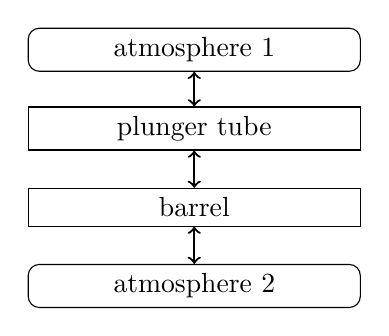
\begin{tikzpicture}
\tikzstyle{cv}       = [rectangle, minimum width=12em, text centered, draw=black]
\tikzstyle{cv_const} = [rectangle, rounded corners, minimum width=12em, text centered, draw=black]
\tikzstyle{arrow}    = [thick, <->]

\node (atm1)        [cv_const]                  {atmosphere~1};
\node (plungertube) [cv, below of=atm1]         {plunger~tube};
\node (barrel)      [cv, below of=plungertube]  {barrel};
\node (atm2)        [cv_const, below of=barrel] {atmosphere~2};

\draw [arrow] (atm1)        -- (plungertube);
\draw [arrow] (plungertube) -- (barrel);
\draw [arrow] (barrel)      -- (atm2);
\end{tikzpicture}
\caption{Abstract connected control volume view of a springer blaster.}
\label{fig:springer control volumes}
\end{figure}

\subsection{\texttt{springer} namelist group variables}

The following variables are in the springer namelist group.
If there is a corresponding typeset variable, the notation for that variable is also listed.

\input{geninput_springer.tex}

\section{Pneumatic mode}
% TODO

\section{BlasterSim internal model}
% TODO

Internally, BlasterSim simulate blasters using control volumes with arbitrary flow connections between control volumes.
This allows BlasterSim to simulates spring and pneumatic blasters with the same core simulation code. This also allows simulating more atypical blasters without major code changes.
